% =====================================================================
%  The temporal recency kernel used by the assimilation loop.
%
%  w(d) = 1                              if d <  D0
%       = (1 + ln(d/D0)/tau)^(-alpha)    if d >= D0
%  with d = t_now - t_i the age of an observation.
%
%  Eq. (2) of Shakouri, Kiriazes & Massoudieh (2026). Parameters as used
%  there: D0 = 30 d, tau = 1, baseline alpha = 1, forgetful alpha = 6.
%  Reproduces the paper's quoted half-weights (82 d and 34 d) and its
%  w(4 yr) ~ 0.2 for the baseline kernel.
%
%  Build: pdflatex fig_kernel.tex && cp fig_kernel.pdf figures/N11_kernel.pdf
% =====================================================================
\documentclass[border=4pt]{standalone}
\usepackage[T1]{fontenc}
\usepackage{helvet}
\renewcommand\familydefault{\sfdefault}
\usepackage{tikz}
\usepackage{pgfplots}
\pgfplotsset{compat=1.18}

\definecolor{ohqblue}{HTML}{1F5C8B}
\definecolor{ohqteal}{HTML}{2A9D8F}
\definecolor{ohqrust}{HTML}{E76F51}
\definecolor{ohqgrey}{HTML}{6B7280}

\begin{document}
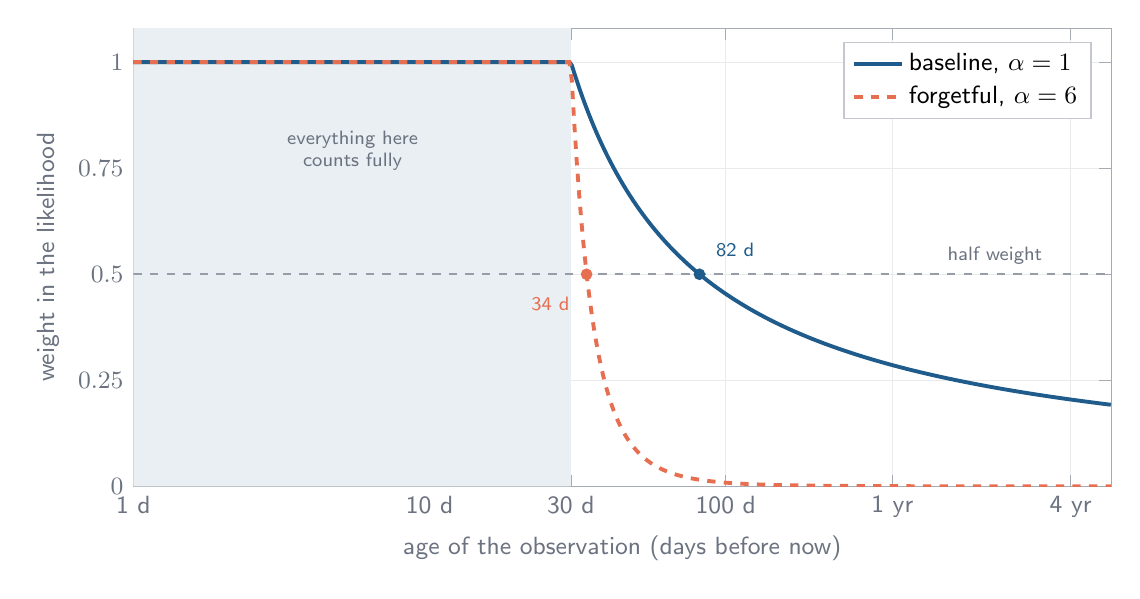
\begin{tikzpicture}[font=\sffamily]
\begin{axis}[
  width=14cm, height=7.4cm,
  xmode=log, domain=1:2000,
  xmin=1, xmax=2000, ymin=0, ymax=1.08,
  xlabel={age of the observation (days before now)},
  ylabel={weight in the likelihood},
  label style={font=\small, text=ohqgrey},
  tick label style={font=\small, text=ohqgrey},
  axis line style={ohqgrey!60}, tick style={ohqgrey!60},
  grid=major, major grid style={ohqgrey!15},
  xtick={1,10,30,100,365,1460},
  xticklabels={1 d, 10 d, 30 d, 100 d, 1 yr, 4 yr},
  ytick={0,0.25,0.5,0.75,1},
  legend style={font=\small, draw=ohqgrey!40, at={(0.98,0.97)},
                anchor=north east, fill=white},
  legend cell align=left,
]

% the flat-weight horizon
\addplot[draw=none, fill=ohqblue!10, forget plot]
  coordinates {(1,0) (30,0) (30,1.08) (1,1.08)} \closedcycle;
\node[font=\scriptsize, text=ohqgrey, anchor=north, align=center]
  at (axis cs:5.5,0.86) {everything here\\counts fully};

\addplot[ohqblue, line width=1.4pt, samples=400]
  {ifthenelse(x<30, 1, (1+ln(x/30))^(-1))};
\addlegendentry{baseline, $\alpha=1$}

\addplot[ohqrust, line width=1.4pt, dashed, samples=400]
  {ifthenelse(x<30, 1, (1+ln(x/30))^(-6))};
\addlegendentry{forgetful, $\alpha=6$}

% half-weight markers
\draw[ohqgrey!70, dashed, line width=0.7pt]
  (axis cs:1,0.5) -- (axis cs:2000,0.5);
\node[font=\scriptsize, text=ohqgrey, anchor=west] at (axis cs:520,0.545)
  {half weight};
\addplot[only marks, mark=*, mark size=1.9pt, ohqblue, forget plot]
  coordinates {(81.5,0.5)};
\addplot[only marks, mark=*, mark size=1.9pt, ohqrust, forget plot]
  coordinates {(33.9,0.5)};
\node[font=\scriptsize, text=ohqblue, anchor=south west] at (axis cs:86,0.52)
  {82 d};
\node[font=\scriptsize, text=ohqrust, anchor=north east] at (axis cs:32,0.47)
  {34 d};

\end{axis}
\end{tikzpicture}
\end{document}
